\documentclass[twoside, 12pt]{article}
\usepackage[utf8]{inputenc}

%THIS IS WHERE ALL THE SYDE STUFF IS
\usepackage{sydestyle}

% Other imports go here
\usepackage{graphicx}
\graphicspath{{figures/}}
\usepackage{amsmath}

% Fill in this blob

\title{Design of a Latex WTR Following the SYDE Guide}
\author{Erik Derohanian}
\studentnumber{12345678}
\lastsemester{3A}
\date{January 12, 1978}
\employer{Gandalf Technologies}
\employeraddress{130 Colonnade Road \\ Nepean, ON K2E 1B6}



% Content here
\begin{document}

	% Start with a title page!
	\makewtrtitle

	% Your letter of submittal should go here:
	Dear prof person,

	Pretend this page is a letter of submittal.

	Erik Derohanian

	12345678

	% new page at the end of the letter.
	\newpage

	% Abstract
	\begin{abstract}
		This is a \LaTeX\ style that aims to match the uWaterloo SYDE style guide because doing work term report formatting makes me want to ahkerfg kasjrgu dfhgukia rgfzjkxfh aeguxdfgzxyu auisdrjgfh ifawuiegf isdurgfia uewrzcjbn zkjdfcvmba weukirydfui erjk t  zxcg awr sdfh stry sdfh yukstrh f nynyuikjef acse fcvdt ukyivegt hac erctse rgc.
	\end{abstract}

	% Make a table of contents.
	\tableofcontents
	\newpage

	% List of figures and tables.
	\listoffigures
	\newpage
	\listoftables
	\newpage

	% Couldn't figure out how to automate this, but leave this line in to restart page numbers at 1 and with arabic numbers.
	\startarabicpagenumbers

	\section{First section}

	Your text goes here. I'm going to add a bunch of words to make this a paragraph longer than one line.

	The next paragraph is automatically indented, as per the guide (default \LaTeX\ behaviour)

	\subsection{A subsection}

	More text.

	\subsubsection{A sub-subsection}

	Yep, it's actually a \textbackslash subsubsection\{sub-subsection name\}.

	\section{Some Tables and Figures}

	Here is a figure:

    \begin{figure}[!ht]
        \centering
        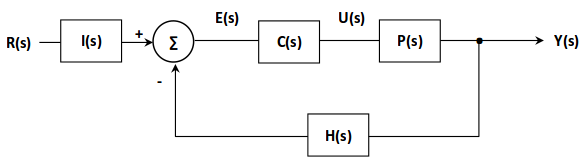
\includegraphics[width=0.7\textwidth]{pcontroller}
        \caption{System diagram of a P controller}
        \label{pcontroller}
    \end{figure}

	I can start talking about that figure, and refer to it as figure \ref{pcontroller} and the number will update based on the label which is very useful when you're shuffling stuff around because you don't have to keep track of figure numbers.

	We can also do tables, like so

	\begin{center}
		\begin{table}[!ht]
		    \begin{tabular}{ | l | l | l | p{5cm} |}
		    \hline
		    Day & Min Temp & Max Temp & Summary \\ \hline
		    Monday & 11C & 22C & A clear day. \\ 	\hline
		    Tuesday & 9C & 19C & Cloudy with rain.\\ \hline
		    Wednesday & 10C & 21C & Rain. \\
		    \hline
		    \end{tabular}
			\caption{Some table I copied from the Latex wikibook online}
			\label{shittytable}
		\end{table}
	\end{center}

	Like the previous figure, we can refer to this table as table \ref{shittytable}.

	Here is a kitten:

    \begin{figure}[!ht]
        \label{kitten}
        \centering
        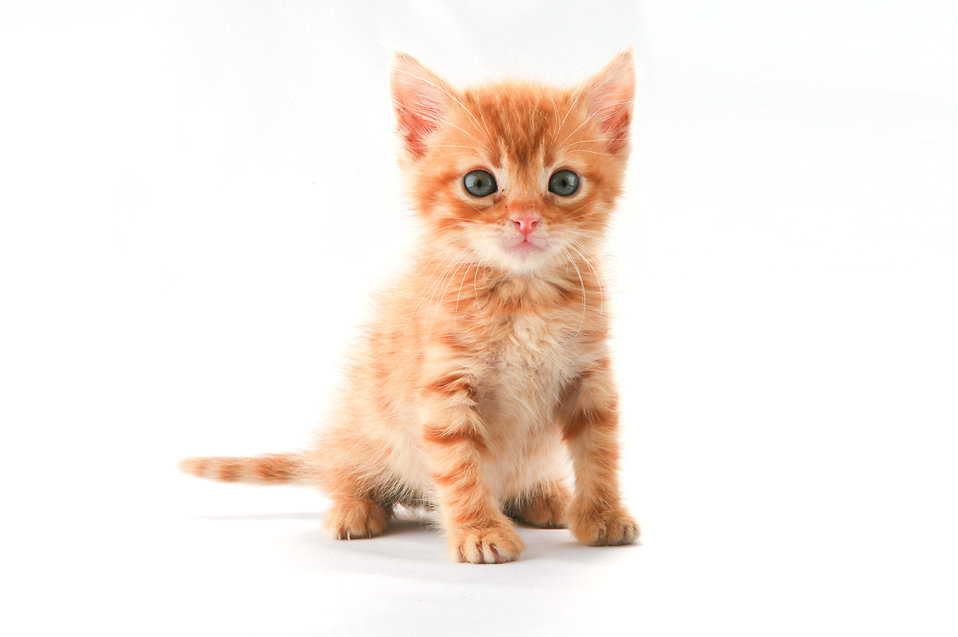
\includegraphics[width=0.5\textwidth]{kitten}
        \caption{It's a kitten. You like kittens.}
    \end{figure}

	\section{Equations}

	Here is the transfer function to the control system shown in figure \ref{pcontroller}:

    \begin{equation}
        \label{ptransfer}
        T(s)=\frac{Y(s)}{R(s)}=I(s) \cdot \frac{K_p \cdot P(s)}{1 + K_p \cdot P(s) \cdot H(s)}
    \end{equation}

	As usual, we can use it's number. That was formula \eqref{ptransfer}

	\section{Citations}

	Three items are cited: \textit{The \LaTeX\ Companion} book \cite{latexcompanion}, the Einstein journal paper \cite{einstein}, and the Donald Knuth's website \cite{knuthwebsite}. The \LaTeX\ related items are \cite{latexcompanion,knuthwebsite}.

	\bibliographystyle{unsrt}%Used BibTeX style is unsrt
	\bibliography{references}

\end{document}
